\section{Business Model Canvas}
\label{BMC_Kapitel}
Die \ac{BMC} bezeichnet ein Geschäftsmodellkonzept. \citeA[S. 14]{BusinessModelGeneration} definieren ein Geschäftsmodell wie folgt:
\begin{quote}
,,Ein Geschäftsmodell beschreibt das Grundprinzip, nach dem eine Organisation Werte schafft, vermittelt und erfasst.''
\end{quote}
Danach entwickelt er ein Muster, welches die Beschreibung eines Geschäftsmodells vereinfachen soll. Unter einer Canvas versteht man hier eine übersichtliche Darstellung der wichtigsten Informationen, nach Möglichkeit von dem Umfang einer Seite. So gliedert sich der Aufbau im Allgemeinen in zwei Hälften. Die rechte Seite der \ac{BMC} beschäftigt sich mit dem Wert der Organisation, wohingegen die linke Seite auf die Effizienz eingeht. Damit ist bereits auf einem Dokument ersichtlich, wie das Projekt effizient Werte vermitteln soll. Im Detail ist die \ac{BMC} in neun Bausteine aufgeteilt, welche in Abbildung \ref{fig:BMC_Structure} dargestellt sind. Auf dieser Darstellung ist erkennbar, dass die rechte Seite auf den Wert für den Endnutzer abgestimmt ist, wohingegen sich die linke Seite auf die Verlagerung von Ressourcen spezialisiert, also die Effizienz, nach \citeauthor{BusinessModelGeneration}. 
\begin{figure}
	\begin{center}
		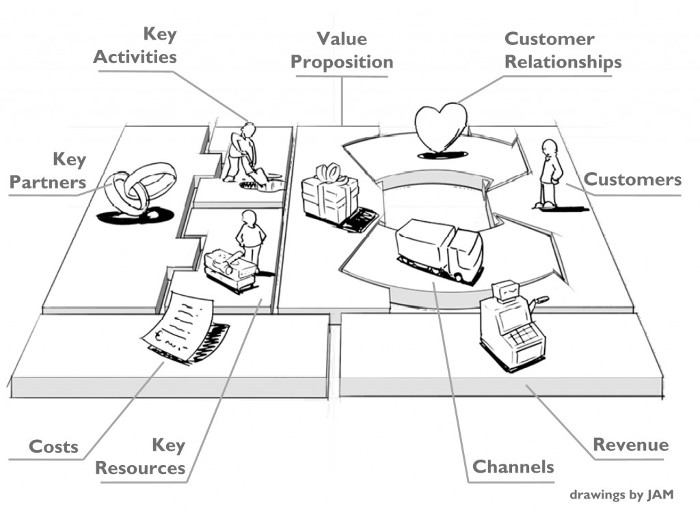
\includegraphics[scale=0.5]{99_IMG/02_Grundlagen/bmcStructure.jpg}
		\caption[Struktureller Aufbau der \ac{BMC}.]{Struktureller Aufbau der \ac{BMC} (Abbildung übersetzt aus \citeNP{Sammer2018}).}
		\label{fig:BMC_Structure}
	\end{center}
\end{figure}
Die einzelnen Bausteine werden im Folgenden genauer erklärt.

\begin{itemize}
	\item \textbf{\ac{CS}}
	
	Die Kundensegmente beschreiben alle Kundengruppen des Unternehmens. Dabei ist es möglich, dass der Massenmarkt die Zielgruppe beschreibt. Zielt ein Produkt allerdings nur auf eine bestimmte Art von Kunden mit ähnlichen Bedürfnissen und Wünschen ab, nennt sich das Nischenmarkt. Darüber hinaus können Kundengruppen segmentiert werden, wenn unterschiedliche Gruppen der gesamten Kundenmenge verschiedene Eigenschaften aufweisen, welche das Kauf- oder Nutzverhalten bestimmen kann. 
	
	\item \textbf{\ac{VP}}
	
	Die Werte, die das Produkt dem Endkunden bringt, werden hier als Wertangebote bezeichnet. Dabei kann in quantitative, also messbare, und qualitative Werte unterschieden werden. Genauer unterscheidet \citeauthor{BusinessModelGeneration} hier in die folgenden Kategorien: Neuheit, Leistung, Anpassung an Kundenwünsche, die Arbeit erleichternd, Design, Marke/Status, Preis, Kostenreduktion, Risikominderung und Verfügbarkeit. Dies sind Beispielkategorien, was bedeutet, dass durchaus auch andere Werte hier gelistet werden können. Die genannten stellen eine Aufzählung der häufigsten Vorteile dar, welche auf die meisten Produkte anwendbar sind. Allerdings ist diese Aufzählung, wie bereits erwähnt, nicht vollständig und darf nicht als solche angesehen werden. 
	
	\item \textbf{\ac{CH}}
	
	Über welche Kanäle das Produkt dem Kunden vermittelt werden soll, wird in diesem Abschnitt dargestellt. Diese können in eigene und Partnerkanäle, sowie direkte und indirekte Kanäle unterschieden werden. Eigene direkte Kanaltypen stellen beispielsweise eine eigene Verkaufsabteilung oder direkter Verkauf über eine eigene Website dar. Dazu bietet eine eigene Filiale einen eigenen, aber indirekten Kanal, da der Verkauf über einen Mittelmann, die Filiale, stattfindet. Indirekte Partnerkanäle sind etwa Partnerfilialen oder Großhändler. Ein Kanal verfügt nach \citeauthor{BusinessModelGeneration} über fünf Phasen. So muss zuerst die Aufmerksamkeit des Kunden erregt werden und diesem die Möglichkeit gegeben werden, das Produkt für sich zu bewerten. Darauf aufbauend soll der Kunde zum Kauf angeregt werden. Nach dem Kauf muss dem Nutzer der Wert des Produktes vermittelt werden und dieser muss auch weiterhin Unterstützung von Seiten des Unternehmens genießen können. Diese Schritte soll ein Kanal im Allgemeinen abdecken können, unabhängig von der Art dessen.
	
	\item \textbf{\ac{CR}}
	
	Die Art von Beziehungen, die ein Unternehmen mit den Kunden eingeht, wird unter \acs{CR} festgehalten. So kann ein Betrieb persönliche Unterstützung anbieten, was häufig an der Verkaufsstelle passiert. Geht diese Unterstützung tiefer ins Detail, kann dies auch \textit{Individuelle Persönliche Unterstützung} genannt werden. Darüber hinaus nennt der Autor Selbstbedienung und Automatisierte Dienstleistungen als Arten von Kundenbeziehungen. Ersteres bezeichnet ein Unternehmen, welches keine direkte Kundeninteraktion führt, sondern den Kunden die Möglichkeit gibt, sich selbst zu bedienen. Diese Art der Kundenorientierung in Kombination mit automatisierten Prozessen wird Automatisierte Dienstleistung genannt. Des Weiteren kann ein Betrieb darauf setzen, die Kunden untereinander in einer Community zu vernetzen. Ein weiterer Weg, Beziehungen zu Kunden aufzubauen, kann es sein, diese zur Mitbeteiligung anzuregen, beispielsweise durch die Aufforderung zu Rezensionen.
	
	\item \textbf{\ac{Rdollar}}
	
	Die Einnahmequellen beschreiben die Umsatzart, die ein Unternehmen anstrebt. Die häufigsten Arten werden hier in folgende Bereiche unterteilt: Verkauf von Wirtschaftsgütern, Nutzungsgebühr, Mitgliedsgebühren, Verleih/Vermietung/Leasing, Lizenzen, Maklergebühren und Werbung. Außerdem wird in Festpreise und variable Preise unterschieden. Ein Festpreis kann sich dabei durch bestimmte Produkteigenschaften, dem Kundensegment oder die Menge zusammensetzen. Allerdings ändert sich dieser nicht durch andere Einflüsse. Im Gegensatz dazu verändert sich ein variabler Preis beispielsweise durch Verhandlungen oder Auktionen. Dazu ist es möglich, dass der Echtzeitmarktwert, also das Zusammenspiel von Angebot und Nachfrage, oder das Ertragsmanagement, abhängig von Bestand und Kaufzeitpunkt, den Preis beeinflussen.
	
	
	\item \textbf{\ac{KR}}
	
	Unter diesem Punkt werden sämtliche Wirtschaftsgüter gelistet, welche für das Unternehmen benötigt werden. Dazu zählen beispielsweise physische Güter, wie Räumlichkeiten oder Maschinen. Außerdem kann eine Ressource auch menschlicher Art sein. Dabei soll besonders auf die Kompetenzen der Kraft eingegangen werden. Auch finanzielle Mittel können hier von Bedeutung sein.
	
	\item \textbf{\ac{KA}}
	
	Die Schlüsselaktivitäten umfassen alle Tätigkeiten, die benötigt werden, damit das Geschäftsmodell funktionieren kann. Unter Anderem können diese Aktivitäten die Produktion einer Ware, die Lösung eines Problemes oder die Vernetzung der Kunden beinhalten. Allgemeiner gefasst wird in diesem Abschnitt aufgezählt, was der Betrieb genau macht, damit der Nutzer von dem Wertangebot profitieren kann.
	
	\item \textbf{\ac{KP}}
	
	Häufig werden Geschäftspartner benötigt, um das Geschäftskonzept umzusetzen, welche unter diesem Punkt aufgeführt werden. \citeauthor{BusinessModelGeneration} unterteilt diese in drei Kategorien. Die erste Gruppe dient der Optimierung oder einem Mengenvorteil. Darunter versteht man beispielsweise die Zulieferung von Bauteilen oder das Auslagern von Infrastruktur. Eine weitere Partnerschaftskategorie dient der Minderung von Risiken und Unsicherheiten. Nicht selten kommt es vor, dass Konkurrenten zusammen an einer neuen Technologie forschen. Dabei kommt diese Art von Partnerschaft zustande. Die dritte Gruppe bildet die Akquise bestimmter Ressourcen und Aktivitäten. Hier werden etwa Kompetenzen oder Lizenzen anderer Unternehmen benötigt, um das eigene Produkt herzustellen.
	
	\item \textbf{\ac{Cdollar}}
	
	Abschließend werden die Kosten aufgelistet, welche mit dem Geschäftsmodell verbunden sind. Dabei kann es unter Umständen sinnvoll sein, zwischen einer kostenorientierten oder wertorientierten Kostenstruktur zu unterscheiden. Kostenorientiert bedeutet hier, dass der Fokus des Unternehmens darauf liegt, die Ausgaben zu senken. Im Gegensatz dazu liegt der Schwerpunkt eines wertorientierten Geschäftsmodells darin, dem Kunden maximalen Wert zu vermitteln. Der Autor nennt hier beispielhaft eine Billigfluglinie als rein kostenorientiertes und ein Luxushotel als wertorientiertes Unternehmen. Meist liegt das Geschäftskonzept zwischen diesen Kategorien. Nichtsdestotrotz können die anfallenden Kosten auch andere Merkmale aufweisen. Hier kann etwa in Fix- oder variable Kosten unterschieden werden. Fixkosten ändern sich nicht, wohingegen variable Kosten etwa von der Menge der produzierten Waren abhängig sind. Außerdem sollten Mengen- und Verbundvorteile beachtet werden. Je mehr Waren ein Unternehmen produziert, desto geringer sind die anfallenden Kosten pro Produkt in der Regel. Dazu kann ein großer Betrieb davon profitieren, mehrere Produkte mit derselben Strategie zu vermarkten, was wiederum Kosten spart.
	
\end{itemize}

Diese Bausteine fassen das Geschäftsmodell prägnant zusammen, sodass mithilfe der Canvas die wichtigsten Details auf einen Blick erkennbar sind.
\cite[S. 13-51]{BusinessModelGeneration}